Dieses Kapitel beschäftigt sich mit der Theorie aller verwendeten Klassifikatoren. Es wird aufgrund der Resultate des logistischen Modells argumentiert, dass die Datenauswahl weitgehend sinnvoll ist. Abschnitt 3.4 führt zudem die Ideen der verwendeten Cross Validation Strategien auf, mit denen die Performance der Modelle verglichen wurde. 

\subsection{Das logistische Modell}
Als Basismodell an dem die Performance der beiden anderen Classifier gemessen werden sollte, wurde ein logistisches Modell geschätzt. Das logistische Regressionsmodell entsteht aus dem Wunsch heraus, die Posteriorwahrscheinlichkeiten der K Klassen über lineare Funktionen im Predictorspace zu modellieren und gleichzeitig sicherzustellen, dass sie zu eins summieren und innerhalb des Intervalls [0,1] bleiben. \cite{logit}
Existieren nur zwei verschiedene Klassen in den Daten, zum Beispiel Sites und Nonsites, so lässt sich das logistische Modell mit nur einer linearen Funktion spezifizieren. Dem sog. linearen Prädiktor $\eta$. \\
\begin{equation}
    \eta = \beta_{\text{0}} + \beta_{\text{1}} \cdot {\text{Höhe}}  + \beta_{\text{2}} \cdot  {\text{Temp}}  + ... + \beta_{\text{p}} \cdot {\text{Hangausrichtung}} 
\label{eqlogit}
\end{equation}
Dabei gilt aus der Konstruktion von $\eta$ über die logarithmierten Chancen (log-odds):\\ 
\begin{equation}
\log \frac{\operatorname{Pr}(K=1 | X=x)}{\operatorname{Pr}(K=2 | X=x)}= \eta
\label{logodds}
\end{equation}
So müssen die aus dieser Konstruktion erhaltenen Koeffizienten anhand der log-odds, oder nach Exponentieren von $\eta$ anhand der Odds interpretiert werden. An dieser Stelle sollte angemerkt werden, dass es in dieser Arbeit nicht im Focus lag die Modelle optimal an die Daten anzupassen, um die zugrunde liegenden datengenerierenden Prozesse bestmöglich zu erklären. Daher wurden die Prädiktoren nur einzeln, als lineare Terme frei von Interaktionen in die Modelle aufgenommen. Die Resultate des logistischen Modells befinden sich in der folgenden Tabelle. 
\begin{table}[htb]
\centering
\begin{tabular}{llllll}
\hline
               & Estimate   & Sig. & Hangrotation & Estimate   & Sig.\\
Intercept      & -1.171e+01 & ***       & Nordost      & -1.591e-01 & *         \\
DEM            & -1.231e-03 & **        & Ost          & -3.988e-01 & ***       \\
Temperatur     & 1.421e+00  & ***       & Südost       & -1.568e-01 & *         \\
Niederschlag   & -4.150e-03 & ***       & Süd          & -2.733e-01 & ***       \\
Gewässer Dist. & -3.102e-05 & ***       & Südwest      & -3.438e-01 & ***       \\
Frosttage      & 2.612e-01  & ***       & West         & -1.876e-01 & *         \\
Sonnenstunden  & 6.659e-01  & ***       & Nordwest     & -8.278e-02 &           \\
TPI            & 1.787e-03  &           &              &            &           \\
Hangneigung    & -1.378e-01 & ***       &              &            &           \\
\hline
\end{tabular}
\caption{Geschätzte Koeffizienten des Logit-Modells. Nonsites und Sites sind als 0/1-kodierte Variable in das Modell eingeflossen. Sig. Codes: 0 ‘***’ 0.001 ‘**’ 0.01 ‘*’ 0.05 }
\label{tab:basefitcoeffs}
\end{table} \\
Im Allgemeinen lassen sich die geschätzten Koeffizienten am schnellsten über ihre Vorzeichen interpretieren. Ein negatives Vorzeichen bedeutet, dass, ceteris paribus, ein Steigen der entsprechenden Kovariable eine Senkung der log-odds für Klasse 1 (hier Sites) zur Folge hätte. Dies ist hier für die Variablen Hangneigung, Gewässerdistanz, Niederschlag, DEM (Höhe über N.N.) der Fall und erscheint bei einem Blick auf die Prediktorkarten in Abbildung \ref{predictorstack} und die geographischen Häufungen der Sites durchaus sinnvoll. So würde man erwarten, dass bei Annäherung an die Alpen -- also Steigern der Höhe, die Chancen bei einer Ausgrabung fündig zu werden sinken. Ein positives Vorzeichen bedeutet hingegen, dass eine Steigerung der entsprechenden Kovariable eine Steigung der log-odds für Klasse 1 (Sites), unter Konstanthalten der anderen Variablen, zur Folge hätte. Dies ist hier sowohl für die Anzahl durchschnittlicher Sonnenstunden pro Tag pro Jahr, als auch für die durchschnittliche Anzahl Frosttage pro Jahr der Fall. (TPI hat mit einem p-Wert von weit über 5\% keinen signifikant von 0 verschiedenen Einfluss auf die log-odds.) Interessant ist auch, dass alle Hangrotationskoeffizienten ein negatives Vorzeichen besitzen. Dies könnte unter Umständen aus dem Zusammenhang von Hangrotation, Hangneigung und Höhenmodell erklärt werden. So können nur an Stellen an denen das Höhenmodell Hänge besitzt Werte für die Hangrotation ermittelt werden. Um diesen Zusammenhang zu klären, sollten noch weitere Untersuchungen durchgeführt werden. \\
Insgesamt scheint die Variablenauswahl sinnvoll, nur der TPI ist trotz der Stichprobengröße von mehr als 12000 Sites und Nonsites nicht signifikant. 
Anmerkung: Während die logit-Transformation des linearen Prädiktors häufig mit der sigmoiden Form der logistischen Funktion in Verbindung gebracht wird, sollte nicht unerwähnt bleiben, dass die logistische Regression zur Klassifikation den Prädiktorraum je nach festgelegter Entscheidungsgrenze mit einer Hyperebene in (in diesem Fall) zwei Klassengebiete unterteilt. \cite{trenngerade} Dies soll mit Abbildung \ref{trenngerade} veranschaulicht werden. 

\begin{figure}[H]
    \centering
    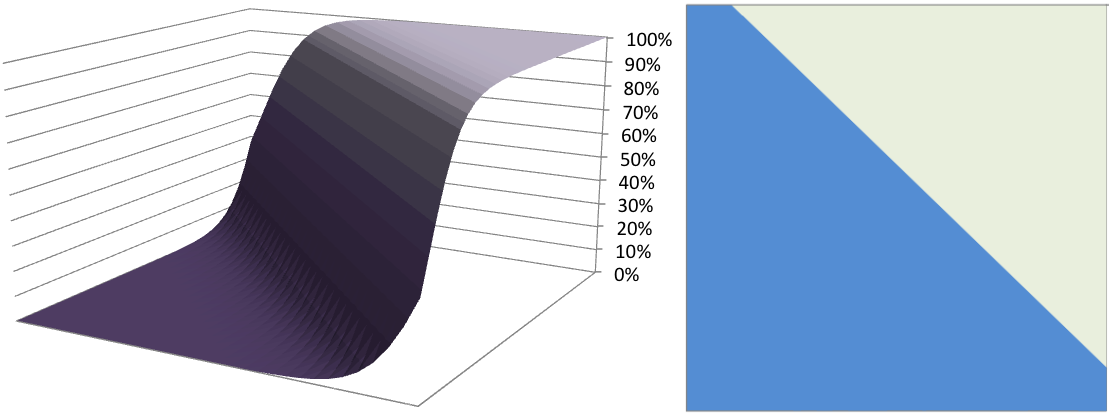
\includegraphics[width = 13cm, height = 7cm]{Figures/trenngerade.png}
    \caption{Logistische Regression mit zwei Kovariablen. Links: Sigmoide Form der auf zwei Variablen angepassten logistischen Funktion. Rechts: Lineare Trenngerade bei einer Entscheidungsgrenze von 50\%. \cite{trenngerade}}
    \label{trenngerade}
\end{figure}

Dieser bemerkenswerte Zusammenhang wirft die Frage auf, ob sich, unabhängig von der Definition über log-odds, lineare Trennebenen im vieldimensionalen Prädiktorraum finden lassen. Der nächste Abschnitt beantwortet diese Frage und führt sog. Kernel-Methoden ein um diese Methoden auf den nicht linear trennbaren Fall auszuweiten.

\subsection{Support Vector Machines}
\subsubsection{Linear separierende Hyperebenen}
Es ergibt sich, dass via logistischer Regression eine lineare Trennebene zur Klassifikation ermittelt werden kann. Dieser Abschnitt befasst sich mit der Konstruktion von linearen Hyperebenen zur Klassentrennung. Dieses Verfahren versucht die Daten so optimal wie möglich in verschiedene Klassen zu zerlegen. Es bildet die Grundlage für Support Vector Classifier. \cite{hyperplanes}\\
Sei L eine Hyperebene definiert durch die Gleichung
\begin{equation}
    f(x)=\beta_{0}+\beta^{T} x=0
\label{eqhyperplane}
\end{equation}
Im zweidimensionalen Fall ergibt sich eine Trenngerade. Es lässt sich zeigen:
\begin{enumerate}
    \item Für beliebige Punkte $x_{1}$ und $x_{2}$ in L gilt: $\beta^{T}\left(x_{1}-x_{2}\right)=0$ und daher ist der Normalenvektor von L gegeben durch: $\beta^{*}=\beta /\|\beta\|$
    \item Für jeden Punkt $x_{0}$ in L gilt: $\beta^{T} x_{0}=-\beta_{0}$
    \item Der Abstand eines punktes $x$ zu L ist gegeben durch: \\
    $\beta^{* T}\left(x-x_{0}\right)=\frac{1}{\|\beta\|}\left(\beta^{T} x+\beta_{0}\right)=\frac{1}{\left\|f^{\prime}(x)\right\|} f(x)$
\end{enumerate}
Daher ist $f(x)$ proportional zum Abstand von $x$ zur Hyperebene definiert durch $f(x)=0$. \cite{hyperplanes}\\
Grundsätzlich versuchen auf Trennebenen basierte Lernalgorithmen die Abstände der fehlklassifizierten Punkte zur Trenngerade zu minimieren. Um diese Abstände optimieren zu können muss allerdings zunächst eine Startebene festgelegt werden. Dies bring jedoch mit sich, dass im linear trennbaren Fall (keine Fehler bei der Klassifikation) mehrere optimale Trennebenen existieren können. Welche gefunden wird hängt von der Startposition ab. Auch würden Algorithmen wie \textit{stochastic gradient descent} im nicht linear trennbaren Fall nicht konvergieren. \cite{hyperplanes} Im Falle von nicht linear separablen Daten lassen sich trotzdem lineare Trennebenen durch Basistransformation der originalen Daten in einen höherdimensionalen Raum konstruieren. Eine einzigartige Lösung lässt sich beispielsweise durch Maximieren der ``Marginbreite'' also des Bereiches um die Trennebene in dem keine Punkte liegen kalkulieren. Dieser Bereich wird vollständig durch die Punkte definiert, welche sich am nächsten an der Ebene befinden. Nach \cite{hastie01statisticallearning} ergibt sich, dass der Lösungsvektor der Ebene als Linearkombination dieser ``Support Points'' definiert werden kann. Dies bildet die Grundlage für die im nächsten Abschnitt diskutierten Support Vector Classifier. 

\subsubsection{Support Vector Classifier}

\begin{figure}[H]
    \centering
    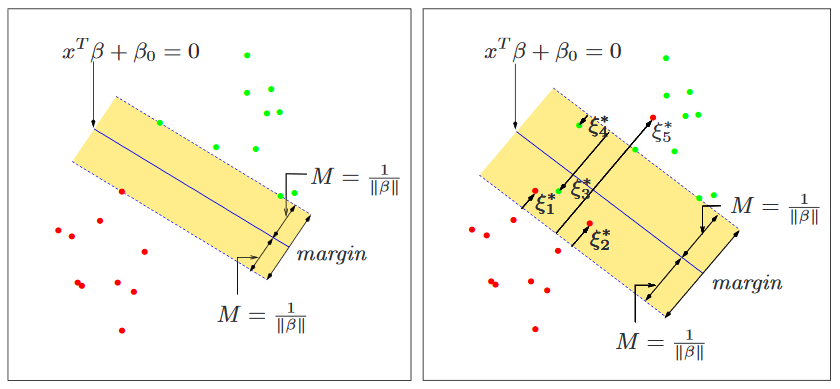
\includegraphics[width = 13cm, height = 7cm]{Figures/svmargin.PNG}
    \caption{Support Vector Classifier. Links: Der im Featurespace linear trennbare Fall. Die Trennebene ist die durchgezogene Linie, während gestrichelte Linien die maximale Margin der Breite $2M=2/\|\beta\|‖$ eingrenzen. Rechts: Der nicht linear trennbare Fall. Die mit $\xi_{j}^{*}$ bezeichneten Punkte befinden sich um einen Betrag $\xi_{j}^{*}= M \xi_{j}$ auf der falschen Seite ihrer Margin. Für Punkte auf der richtigen Seite ist $\xi_{j}^{*}=0$. Die Breite der Margin wird unter der Nebenbedingung $\sum \xi_{i} \leq \text {constant}$ maximiert. $\sum \xi_{j}^{*}$ ist die Gesamtdistanz der Punkte auf der falschen Seite der Trennebene.\cite{svclassifier}}
    \label{svclassif}
\end{figure}

Überlappen sich die Punkte im Featurespace gibt es zwei intuitive Möglichkeiten die Nebenbedingung in \ref{svclassif} zu formulieren. Als erstes könnte die Summe der absoluten Gesamtdistanzen konstant gehalten werden, dies ist aber im Allgemeinen kein konvexes Optimierungsproblem. Daher wird der ``standard'' Support Vector Classifier unter der Randbedingung die proportionalen Anteile der falschen Klassenzuweisungen unter einem Maximum zu halten formuliert. 
\begin{equation}
    \label{eqsvmoptim}
    y_{i}\left(x_{i}^{T} \beta+\beta_{0}\right) \geq M\left(1-\xi_{i}\right)
\end{equation}
Der Wert $\xi_{i}$ in der Nebenbedingung $y_{i}\left(x_{i}^{T} \beta+\beta_{0}\right) \geq M\left(1-\xi_{i}\right)$ entspricht dem relativen Anteil mit dem die vorhergesagte Klasse $f\left(x_{i}\right)=x_{i}^{T} \beta+\beta_{0}$ des Punktes $x_{i}$ von der durch die Entscheidungsgerade geschätzten Klasse abweicht. Daher wird durch Einschränken von $\sum \xi_{i}$ der gesamte relative Betrag, um den Prognosen auf der falschen Seite ihrer Marge fallen, eingeschränkt. Falsche Klassifizierungen treten auf wenn $\xi_{i}>1$ also wird durch Begrenzen der Summe  $\sum \xi_{i}$ die maximale Anzahl von Trainingsfehlern auf den gleichen Wert begrenzt. \cite{svclassifier}

Die optimale Breite der Margin eines Support Vector Classifiers muss unter weiteren Nebenbedingungen wie beispielsweise bestmöglicher Prognoseperformance für unbekannte Daten oder vergleichbaren Kriterien bestimmt werden. Dieser Kostenparameter $C$ ist also verantwortlich dafür, wie stark der Einfluss von weit von der Trennebene entfernten Punkten auf die Lage dieser ist. Große Werte für $C$ optimieren die Trennebene eher für korrekt klassifizierte Punkte nahe der Ebene. Kleinere Werte verstärken eher den Einfluss von Punkten die weiter von der Trennebene entfernt liegen. \cite{svclassifier} \\
Mit welcher Strategie Hyperparameter wie $C$ vor dem Fitten des Modells bestimmt werden, wird in Abschnitt 3.4 erklärt.  

\subsubsection{Kernel-Methoden und Support Vector Machines}

Die bisher beschriebene Support Vector Methodik beschränkt sich auf das Finden linearer Trennebenen im originalen Predictorspace. Werden durch das Berücksichtigen von Punkten innerhalb einer vordefinierten Grenzregion um die Entscheidungsebene auch nicht komplett linear trennbare Fälle schätzbar, so existieren weiterhin eine Vielzahl von möglichen Datensituationen in denen ein einfacher SV-Classifier an seine Grenzen stößt. \\
Wie mit anderen linearen Modellen lässt sich die Methodik des SV-Classifiers durch Basistransformationen des Predictorspace erweitern. Diese Idee wird in Abbildung \ref{kerneltrick} visualisiert. 

\begin{figure}[H]
    \centering
    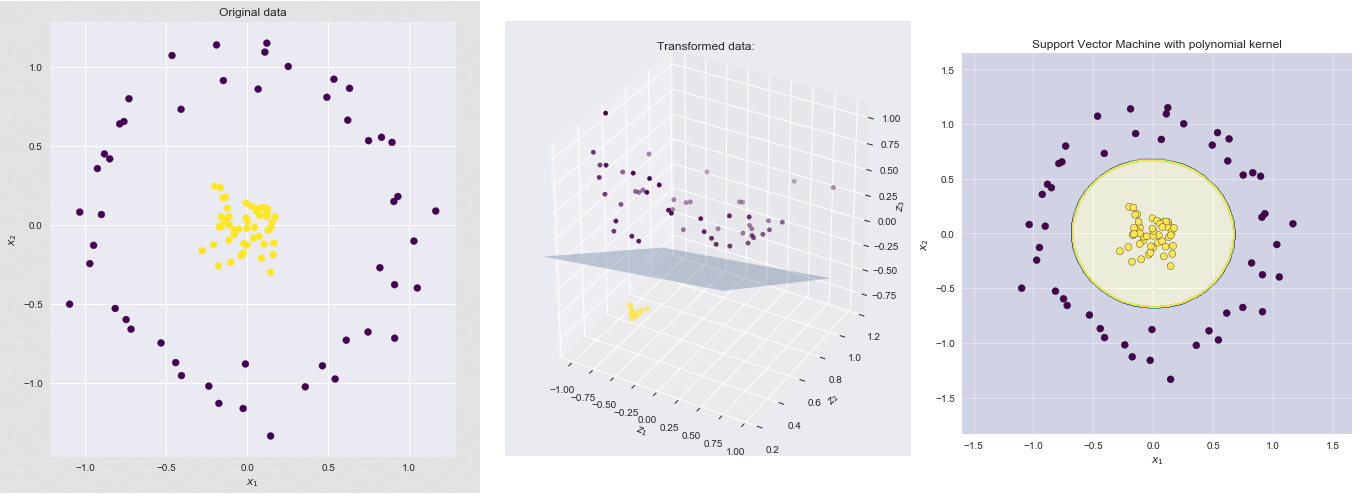
\includegraphics[width = 15cm, height = 6.5cm]{Figures/kerneltrick.png}
    \caption{Nichtlineares Klassifikationsproblem. Die im linken Panel abgebildete Datensituation lässt sich im originalen Predictorspace nicht linear trennen. Die in der Mitte abgebildete Transformation erlaubt die konstruktion eines linearen SV-Classifiers im neuen Prädiktorraum. Rechts ist die Trennlinie zu sehen welche sich durch Retransformieren der linearen Entscheidungsgrenze des 3D Raumes auf den ursprünglichen Prädiktorraum ergibt. \cite{kernelintuition} }
    \label{kerneltrick}
\end{figure}
Um komplexere, nicht-lineare Entscheidungsgrenzen zu erhalten, wird der ``Support Vector Machine'' Algorithmus angewendet. Dieser erlaubt es vieldimensionale Transformationen des Prädiktorraums zu betrachten. (In einigen Fällen kann die Dimension des Predictorspace bis ins Unendliche wachsen.) Dazu ersetzen wir $x$ überall in den bisherigen Formeln durch $\phi(x)$ und wiederholen den Optimierungsprozess. \cite{kernelintuition} Generell wird durch die Transformation der Daten in einen höherdimensionalen Raum die Berechnung von Abständen deutlich aufwendiger als beispielsweise im zweidimensionalen Fall. Um dieses und weitere Probleme zu umgehen, verwendet man für die Transformationen sog. ``Kernel'' oder ``Kern'' Funktionen. Eine intuitive Betrachtungsweise von Kernelfunktionen wäre, dass diese Funktionen entsprechen, welche messen, wie eng die Inputvektoren $x$ und $z$ miteinander verwandt sind. Wenn $x$ und $z$ ähnlich zueinander sind, gibt der Kernel also einen großen Wert aus, und wenn sie ungleich sind, liefert der Kernel kleinere Werte. Dies rechtfertigt die Verwendung eines Gaußkerns für die weitere Analyse. \\
\begin{equation}
    \label{gausskern}
    K(x, z)=\exp \left(-\frac{\|x-z\|^{2}}{2 \sigma^{2}}\right)
\end{equation}
Sind $x$ und $z$ gleich so nimmt der Gausskern den Wert 1 an. Je größer die Differenz von $x$ und $z$, desto mehr nähert sich der Wert des Gausskerns 0 an. \\ Für die Analyse der Eisenzeitfundstellen wurde ein Gausskern verwendet. Die optimale Bandbreite des Kerns ist ein weiterer Hyperparameter, der vor Schätzen des Modells angepasst werden muss. Dieser Parameter $\sigma$ bestimmt die Breite des Kerns, was sich direkt auf die Form der Entscheidungsgrenze auswirkt. Große Werte für $\sigma$ tragen dazu bei, dass die Grenze flexibel ist, was für Prognosemodelle eher ungünstig sein kann, da in solchen Fällen ``overfitting'' vermieden werden sollte.

\subsection{Regression Trees \& Random Forests}

Eine weitere Möglichkeit zur Klassifikation sind Decision Trees. Dieser Abschnitt führt die Theorie von binären Partitionierungen zum Aufbau von Regressions- und Klassifikationsbäumen an und beschäftigt sich mit der Generalisierung dieser Methodik, um robustere Prognoseergebnisse aus den Vorhersagen von Decision Trees zu erzeugen. 

\subsubsection{Regression Trees}

\begin{figure}[H]
    \centering
    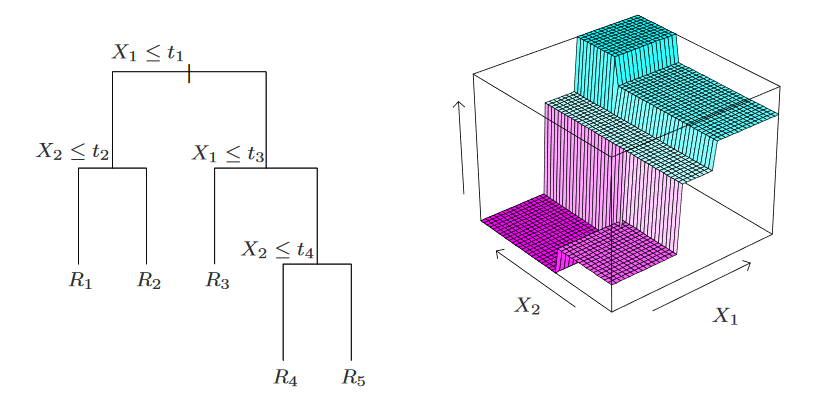
\includegraphics[width = 15cm, height = 6.5cm]{Figures/treesplit.PNG}
    \caption{Regressionsbaum. Links: Ein Beispiel für einen durch rekursive binäre Partitionierung eines zweidimensionalen Prädiktorraums erhaltenen Regression Trees. Rechts: Ein Diagramm der durch diese Einteilung erhaltenen Prognosefläche im Prädiktorraum. \cite{treesplit} }
    \label{treesplit}
\end{figure}

Allgemein lässt sich eine Outcomevariable $Y$ durch Unterteilen des Prädiktorraums in verschiedene Regionen und Zuweisen eines konstanten Wertes $Y^{*}$ zu jeder dieser Regionen modellieren. Da bestmögliche Teilregionen beliebig komplex, und daher schwierig zu charakterisieren, werden können beschränkt sich dieser Ansatz auf rekursive binäre Partitionen, was bedeutet, dass der Prädiktorraum zunächst in zwei Regionen aufgeteilt wird und der Outcome $Y$ mit dem Mittelwert von $Y$ jeder Teilregion modelliert wird. Die Variable nach der aufgeteilt wird, wird einem bestmöglichen Split entsprechend ausgewählt. Dann werden eine oder beide dieser Regionen in je zwei weitere Regionen aufgeteilt, und dieser Prozess wird fortgesetzt, bis eine vordefinierte Regel zum Anhalten in Kraft tritt. \cite{treesplit} Aus diesem Prozess ergibt sich die Baumstruktur im linken Panel von Abbildung \ref{treesplit}. Trotz der Restriktion auf binäre Splits lässt dieses Verfahren, in Abhängigkeit der gewählten Anhalteregel, beliebig viele Aufteilungen des Variablenraumes zu. Der größte Vorteil von Entscheidungsbäumen ist ihre simple Interpretierbarkeit. Das gesamte Modell ist in einem binären Baum enthalten, die einzige Schwierigkeit bildet die Interpretation der Baumstruktur bei vielen Splits und/oder vielen Kovariablen. \\
Für die Klassifikation der Eisenzeitsiedlung stellt sich also die Frage, wie genau der Entscheidungsbaum wachsen sollte um optimale Prognosen zu treffen. Der Datensatz besteht aus einem 2-Klassen Outcome (Sites vs. Nonsites) und 9 Einflussgrößen mit insgesamt über 12000 einzelnen Beobachtungen. Es muss also entschieden werden welche Variablen an welchen Stellen aufgeteilt werden und welche finale Struktur der Baum haben sollte. Angenommen der Prädiktorspace soll in $M$ Regionen $R_{1}, R_{2}, \ldots, R_{M}$ unterteilt werden und der Outcome des Modells wird als Konstante $ c_{m}$ in jeder Region modelliert. 
\begin{equation}
    \label{treemodel}
    f(x)=\sum_{m=1}^{M} c_{m} I\left(x \in R_{m}\right)
\end{equation}
So ergibt sich, ähnlich einem Mittelwertsmodell, der optimale Fit für die Klassifikation als Durchschnitt der Response in jeder der Teilregionen. 
\begin{equation}
    \label{leastsquarestree}
    \hat{c}_{m}=\operatorname{ave}\left(y_{i} | x_{i} \in R_{m}\right)
\end{equation}

Durch Minimieren der quadrierten Abstände der Punkte der Teilregionen zu den Mittelwerten der vorgeschlagenen Klassen lässt sich also für jeden binären Split ein optimaler Wert finden an dem die Aufteilung durchgeführt werden sollte. 
Dieser Prozess wird so lange wiederholt bis die gewünschte Größe bzw. Tiefe des Regressionsbaumes erreicht ist. Wie lange also das Splitting wiederholt werden sollte ist ein Hyperparameter der nicht ohne ein notwendiges Kriterium bestimmt werden kann. Bäume die den Prädiktorraum in zu viele kleine Partitionen unterteilen tendieren dazu, übermäßig viele Informationen aus dem ``Trainingsdatensatz'' zu lernen. Dieses Overfitting führt im Normalfall zu schlechteren Prognoseergebnissen auf ``Testdaten''. Für predictive maps die angeben an welchen Stellen die bayrische Landschaft als Habitat für Menschan aus der Eisenzeit geeignet ist, sind zu tiefe Bäume also eher nicht erstrebenswert. Wie oben erwähnt, besteht der verwendete Datensatz aus etwa 12000 Einträgen, die Prognosekarten werden also auf Basis von über 200000, dem Modell unbekannten, Rasterzellen generiert.\\ Die beste Strategie um einzelne Bäume zu optimieren ist ``cost-complexity pruning'' ein Verfahren, dass zunächst einen ``vollständigen'' Baum $T_{0}$ erzeugt um dann nach einem Teilbaum $T \subset T_{0}$ sucht, der das in \ref{costcomplexity} definierte cost-complexity Kriterium minimiert, also den Tradeoff zwischen Modellfit und Komplexität des Baumes zu optimieren versucht. \\
Sei $m$ die Anzahl an Endpunkten des Baumes $T_{0}$, also die Anzahl der Partitionen $R_{m}$ in die der Baum den Prädiktorraum einteilt. Sei außerdem $N_{m}$ die Anzahl der Beobachtungen $x_{i}$ im Endpunkt $R_{m}$ und $|T|$ die Anzahl der Endpunkte des Teilbaumes  $T \subset T_{0}$.
Mit \\
\begin{equation}
    \label{treecost1}
    \hat{c}_{m}=\frac{1}{N_{m}} \sum_{x_{i} \in R_{m}} y_{i}
\end{equation}
\begin{equation}
    \label{treecost2}
    Q_{m}(T)=\frac{1}{N_{m}} \sum_{x_{i} \in R_{m}}\left(y_{i}-\hat{c}_{m}\right)^{2}
\end{equation}
lässt sich das cost-complexity Kriterium definieren: 
\begin{equation}
    \label{costcomplexity}
    C_{\alpha}(T)=\sum_{m=1}^{|T|} N_{m} Q_{m}(T)+\alpha|T|
\end{equation}

Ziel ist es also, den Baum $T_{\alpha} \subset T_{0}$ zu finden welcher das CC-Kriterium $ C_{\alpha}(T)$ minimiert. Dies wird üblicherweise mit einer Mischung aus ``weakest link pruning'' und Cross Validation bewerkstelligt. \cite{treesplit} für eine detailliertere Erklärung dieser Methoden bzw. 3.4 Für eine Diskussion der verwendeten Verfahren zur Cross Validation. \\
Anmerkung: Das hier beschriebene Vorgehen mit Minimieren der quadratischen Abstände ist nur für Regression Trees geeignet. Für die Klassifikation wird im Normalfall eine Missklassifikationsmaß wie der Missclassification Error oder der Gini-Index minimiert. Der Vollständigkeit halber wurde hier die Konstruktion von Regressionsbäumen beschrieben, allerdings ist das Vorgehen für Klassifikationsbäume, abgesehen von der gewählten ``cost function'' identisch. 

\subsubsection{Random Forest Classifier}

Ein Nachteil einzelner Regressions- bzw. Klassifikationsbäume ist die hohe Variabilität der aus ihnen resultierenden Schätzungen. So kann eine minimale Veränderung im Datensatz eine drastische Veränderung der Baumstruktur zu Folge haben was also einen spürbaren Effekt auf die Prognosen von Trees haben kann. Die am weitesten verbreitete Methode zur Reduktion der Vorhersagevarianz ist ``bootstrapped aggregation'' also das Schätzen und Aggregieren vieler einzelner Entscheidungen auf Bootstrapstichproben. \\
Random forests sind eine Kombination einzelner Baumprädiktoren, so dass jeder Baum von unabhängig und identisch gezogenen Werten eines Zufallsvektors der Daten abhängt. Die durch Generalisieren des Random Forest auf Testdaten erhaltene Fehlerrate konvergiert mit wachsender Stückzahl der Trees im Random Forest fast sicher gegen einen Grenzwert. Dieser Generalisierungsfehler hängt von der Prognosestärke der individuellen Bäume und der Korrelation der Bäume untereinander ab. \cite{randomforest}\\
Grundsätzlich geht man zur Bildung eines Random Forest Classifiers nach dem folgenden Schema vor:
\begin{enumerate}
    \item Ziehe eine Bootstrap Stichprobe der Größe $N$ aus den Daten.
    \item Erzeuge einen Regressions- oder Klassifikationsbaum entsprechend des jeweils benötigten Kriteriums. (Cost Funktion)
    \item Wiederhole Schritte 1 und 2 so lange bis die gewünschte Zahl Bäume erreicht wurde. 
    \item Treffe Prognoseentscheidung für Regression anhand des Durchschnitts der Vorhersagen aller Bäume bzw. anhand der ``Mehrheit der Stimmen'' des Baumensembles für Klassifikation. 
\end{enumerate}
Anmerkung: Eine Prognosekarte die nur die erwarteten Klassen für jede Rasterzelle abbildet wäre im Zweiklassenfall nicht sonderlich hilfreich. Die Softwarepakete ``ranger'' \cite{ranger} und ``randomForest'' \cite{forestpackage} erlauben es allerdings auch die geschätzten Klassenzugehörigkeiten als Wahrscheinlichkeiten auszugeben. So sind auch die zugehörigen Prognosekarten zu Logit-Modell und SVM-Classifier zu interpretieren, wodurch die Karten alle direkt miteinander vergleichbar sind. Weitere Details zu Random Forest Klassifikatoren und Beweise dazu, dass dekorrelierte Baumensembles reduzierte Varianzen besitzen finden sich in \cite{randomforest}. 

\subsection{Hyperparameter Tuning \& Modellperformance}

Um die Klassifikatoren nicht nur visuell oder anhand geschätzter Zelldifferenzen miteinander vergleichen zu können und die Hyperparameter der SVM- und Random Forest Classifier zu bestimmen (tunen) wird üblicherweise 5- oder 10-fold Crossvalidation durchgeführt. Dabei wird der Classifier nur auf einem Teil des Gesamtdatensatzes trainiert und im Anschluss anhand der übrigen Testdaten und einem passenden Performancemaß getestet. Diese Schritte werden beliebig oft unter Variation der Hyperparameter wiederholt um den vordefinierten Parameterraum nach den optimalen Modellparametern zu durchsuchen. Als Maß für die Prognosegüte wurde hier die Fläche unter der ``receiver operating characteristic'' Kurve herangezogen. Diese ermittelt für jede Entscheidungs-Threshold vgl. \ref{trenngerade} im Intervall $[0,1]$ die False-Positive und False-Negative Raten. Die Fläche unter der Kurve kann also als Schätzer für die Gesamtprognosegüte verwendet werden. \\
Herkömmliche CV unterteilt den Datensatz zufällig in Trainings- und Testdaten. Punkte die auf der Erdoberfläche nahe beieinander liegen haben durch die stetige Natur geographischer Einflussgrößen sehr häufig ähnliche Variablenausprägungen. (Orte die nur einige hundert Meter voneinander entfernt sind ähneln sich im Allgemeinen in der Niederschlagsmenge und Durchschnittstemperatur) Dies hat zur Folge, dass bei Crossvalidation der Trainingsdatensatz Informationen über die Testdaten enthält wenn viele Punkte die ursprünglich nahe beieinander lagen in unterschiedliche Sets aufgeteilt werden. Daher wurde für die Modellperformance herkömmliche CV mit ``Spatial'' Cross Validation verglichen. Bei Spatial CV werden die Daten in räumlich zusammenhängende Stücke geteilt welche dann als Test- und Trainingssets verwendet werden. Abbildung \ref{resamplingviz} illustriert die Differenzen beider Methoden. 
\begin{figure}[H]
    \centering
    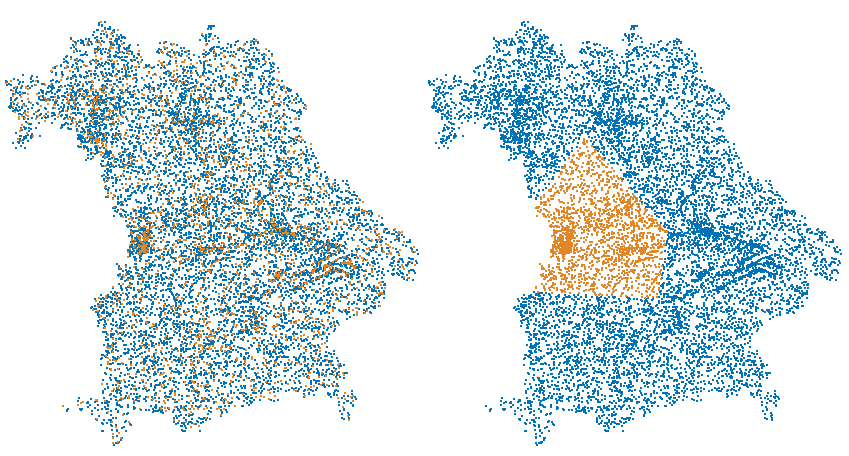
\includegraphics[width = 15cm, height = 6.5cm]{Figures/resampling.png}
    \caption{Resamplingverfahren. Links: Klassische Kreuzvalidierung -- Die Daten werden zufällig in Trainings- (Orange) und Testdaten (Blau) eingeteilt. Rechts: Spatial Cross Validation -- Die Daten werden auch in zwei Sets aufgeteilt, allerdings hängen diese Sets jeweils räumlich zusammen.}
    \label{resamplingviz}
\end{figure}
Eine räumlich zusammenhängende Aufteilung hat zur Folge, dass die Information über das Testset, welche im Trainingsset enthalten ist verringert wird. Also sollte erwartet werden, dass die mittleren Performanceergebnisse mit Spatial CV ein wenig nach unten korrigiert sind. Der Ergebnisvergleich der beiden Verfahren befindet sich in Kapitel 4. \\
Anmerkung: Die Verwendung derselben Daten für die Performanceschätzung und das Hyperparametertuning würde zu überoptimistischen Ergebnissen führen \cite{nestedresmpling2}. Dies kann durch nested Spatial CV vermieden werden. Folgende Grafik verdeutlicht das Vorgehen dabei: 
\begin{figure}[H]
    \centering
    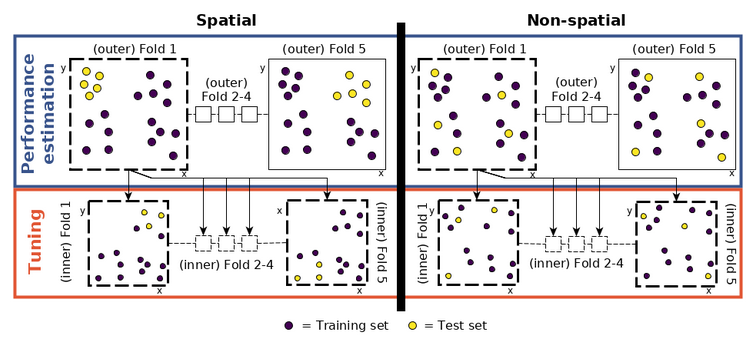
\includegraphics[width = 15cm, height = 6.5cm]{Figures/nestedresampling.PNG}
    \caption{Nested Resampling. Links: Die Unterteilung in räumlich zusammenhängende Stücke der spatial CV. Performance estimation wird auf äußeren Folds durchgeführt, optimale Hyperparameter werden durch erneute Unterteilung der äußeren Folds in Trainings- und Testdaten ermittelt. Rechts: Das gleiche Schema für herkömmliche CV. \cite{nestedresmpling2}}
    \label{nestedresamplingviz}
\end{figure}
